
\setcounter{chapter}{1}

\chapter{Building blocks of situated communicative interactions}
\label{c:building-blocks}

Let us now introduce some of the building blocks that form the basis
of all experiments in this thesis. We will start with a detailed
characterization of the communicative interactions between agents and
how the agents can learn from them. Then we will discuss different
ways of representing linguistic knowledge, i.e. how word forms can be
connected to meanings and what impact the structure of this
association has on the complexity of the learning task. And finally,
we give an overview how word meanings can be grounded in robots, i.e.
how persisting conceptual representations can be constructed by
robotic agents and how they co-evolve with language. For all of these
mechanisms and representational structures we will motivate their
underlying design choices from various perspectives. But we will not
give formal definitions yet and leave that to the description of the
actual experiments later in this thesis.


\section{Language games: the social context}


Following the assumption that communication is a social act in which a
speaker uses language to affect the mental states of a hearer (see
Section \ref{s:communication-as-a-social-act} above) and that a shared
language is constructed and shaped in repeated conversations (Section
\ref{s:language-as-a-complex-adaptive-system}), we will design all of
our experiments around one particular such type of interaction, called
a \emph{language game}. This term is commonly associated to
\cite{wittgenstein67philosophische}, who made an analogy between the
use of language in dialogue and playing a game (e.g. a ball-game; in
both cases there are sets of context-dependent rules for each
interaction step), and it is
\cite{steels95selforganizing,steels01language} who is recognized for
adopting Wittgenstein's concept of language games to the modeling of
communicative interactions between artificial agents.



\subsection{Distributed co-ordination in language games}
\label{s:language-game}

Language games are played by populations of autonomous \emph{agents}
that are modeled as software programs (utilizing standard agent-based
techniques of artificial intelligence, see
e.g. \citealp{wooldridge95intelligent,russel95artificial}). Each agent
maintains its own set of initially empty \emph{inventories}
(e.g. ontologies, lexicons, etc.) for memorizing acquired
knowledge. The agents have built-in mechanisms for using these
inventories to produce and interpret language in a rather automatic
way, \emph{diagnostics} and \emph{repair strategies} for detecting and
overcoming problems in their internal information processing and
\emph{alignment mechanisms} to adapt their inventories in order to
perform better in future interactions. The agents make their own
decisions solely based on internal goals and states, their perception
of the environment and their interaction with others -- i.e. there is
no central control, agents can't directly effect mental states of
others nor have they access to others' mental states (there is no
telepathy) and no agent has an overview over the whole population.

The agents are situated in a \emph{world} to which they are connected
via sensors and actuators. The external goal that is given to the
agents is to communicate about things in the world. Thus, the
environment creates a \emph{communicative task} for the agents and
part of designing an experiment is defining what things in the world
will be presented to the agents. The world is usually not static,
i.e. the configuration of the scenes presented to the agents may
continuously change. As mentioned before, we will investigate models
of lexicon formation both in simulated worlds and with physical robots
in real environments. For our simulated environments will not try to
set up virtual worlds in which simulated robots interact in but we
completely scaffold all problems of perception and categorization by
generating pre-conceptualized scene descriptions that are directly
perceived by the agents. An example scene consisting of two objects
created by such a world generator could look like this: 

\begin{verbatim}
green(obj-1), small(obj-1), square(obj-1), red(obj-2), 
small(obj-2), circle(obj-2)
\end{verbatim}

\noindent In contrast, in our experiments with physical environments,
real robots perceive actual objects through their cameras (see Chapter
\ref{c:embodiment}).


A language game follows a strict script. That is, the agents conform
to routinized dialogue patterns that consist of distinct actions
applicable only to specific contexts and which constrain how to
interpret utterances. An example of such a routinized dialogue is the
procedure for running into a person that one knows: (in western
English-speaking cultures) it starts with a greeting phrase (``hi'',
``hello'', etc.), usually accompanied by eye contact and optionally
complemented by a hand shake or other greeting gestures. Then the
chances are very high that one of the interlocutors will take
initiative and say ``How are you?'', a question which the other person
is not supposed to answer honestly but to reply with ``fine'',
``great'', etc., optionally followed by ``, and you?''  (which doesn't
need be replied). Only after these compulsory steps the two persons
can start to have a real conversation. And it is not OK to end the
dialogue by just going away, it has to be announced (e.g. ``Well, I
have to leave.'') and concluded by a final phrase such as ``see you
later'', ``goodbye'', etc.

Another example is the routine for buying a train ticket at a counter.
After an optional greeting, the customer will utter his
request. Because the ticket seller already knows that the customer
will most likely want to buy a ticket, it is enough to say for
example: ``One ticket to London for tomorrow morning please'' (the
``please'' does not add any information but is compulsory). The seller
will then issue the ticket, if necessary asking for more details. When
the ticket gets printed, the seller will say a price (e.g. ``seventeen
pounds''), which functions (since the customer could also read the
price from the electronic display in front of him) as a request to
hand over the money. The interaction ends with both involved persons
thanking each other and optional greetings.

The type of game that we are going to use for our experiments is not
not embedded in complex activities such as meeting another person on
the street or buying a train ticket. The underlying purpose of the
dialogue lies solely in the communication itself and in providing rich
opportunities for learning and alignment. The game is thus a rather
idealized interaction scenario with only one goal: drawing attention
to an object in the external environment. But it doesn't lack realism:
we will discuss below that children indeed learn many words from such
interactions and it is also very close to one of the games discussed
by \cite{wittgenstein67philosophische}, in which parents teach
children words by pointing at an object and uttering a name for it. A
situation in which somebody points at a thing (e.g. a cow) and tells
its name (e.g. ``cow'') with the purpose of teaching the word to a
child can be conceptualized as a game because in order for the child
to successfully learn the name for the object it has know how the game
works, i.e. that the parent is telling something about the thing that
he is pointing at (it could be also that pointing at a cow and
uttering ``cow'' is an action that the parent performs in order to
make the cow go away or to get milk from it, but that's not the case
-- the game is about learning words and the child has to know this in
order to make sense of the action).

\begin{figure}[t!]
  \centerline{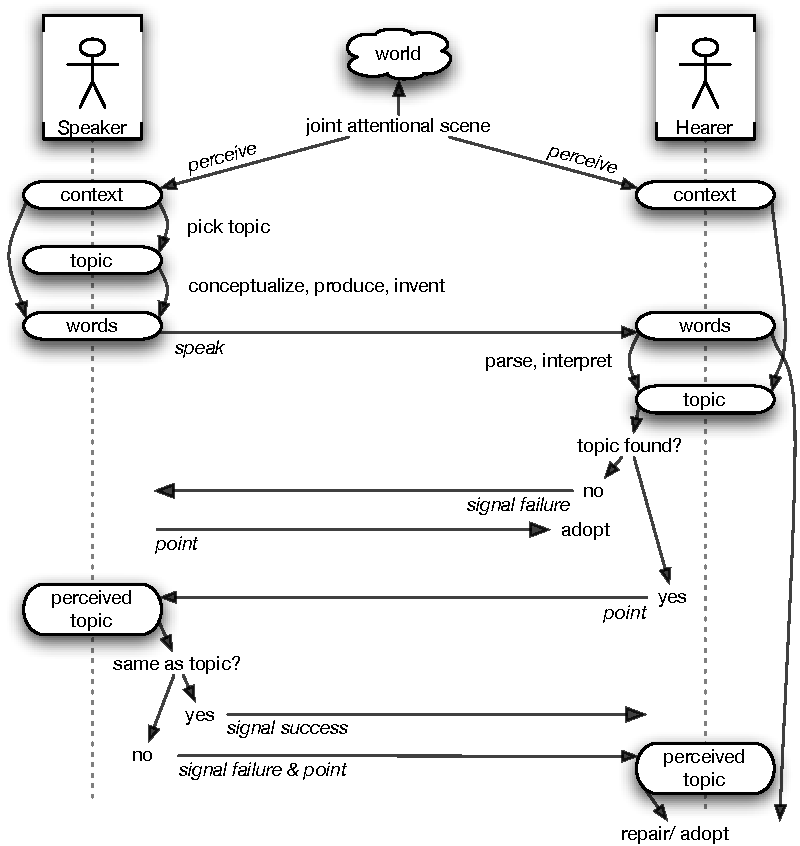
\includegraphics[width=0.85\textwidth]{figures/guessing-game-flow}}
  \caption{Flow of one language game. A speaker and a hearer follow a
    routinized script. The speaker tries to draw the attention of the
    hearer to a physical object in their shared environment.  Both
    agents are able to monitor whether they reached communicative
    success and thus learn from the interaction by pointing to the
    topic of the conversation and giving non-linguistic feedback.
    Populations of agents gradually reach consensus about the meanings
    of words by taking turns being speaker and hearer over thousands
    of such games. }
  \label{f:guessing-game-flow}
\end{figure}


Figure \ref{f:guessing-game-flow} shows a schematic view of the
language game that our agents are going to play (we will discuss each
of mechanisms mentioned below in much more detail in the description
of the actual experiments -- here we only will outline the general
dialogue script that is shared by all experiments throughout this
thesis). Two agents are randomly drawn from the population and
together establish a \emph{joint attentional scene}
\citep{tomasello95jointattention} -- a situation in which both agents
attend to the same set of objects in the environment and in which both
agents know that the respective other agent is attending to the same
set of objects. Once such a state is reached, the game starts. One of
the agents is randomly assigned to take the role of the speaker and
the other the role of the hearer. Both agents perceive then a
\emph{sensory context} from the joint attentional scene and keep it in
their short-term memory (visual perception and joint attention with
real robots is enormously difficult and we will dedicate the whole
Chapter \ref{c:embodiment} to that; in our experiments involving
simulated environments all these issues will be scaffolded and both
agents will perceive the same scene description that is generated by
the world generator mentioned above).

Next, the speaker randomly picks one object from his context to be the
\emph{topic} of the interaction -- his communicative goal will be to
draw the attention of the hearer to that object. For this he
constructs an utterance, which involves first coming up with a mental
representation of the meanings to express (\emph{conceptualization})
and then finding words that cover these meanings. When the speaker
does not have the necessary categories or words in his inventories, he
\emph{invents} them. Additionally, the speaker uses himself as a model
of the hearer and by listening to himself (\emph{re-entrance}), he
checks whether the words he came up with are clear and precise enough
to be understood (given his own inventories). Once the speaker is
satisfied with the constructed utterance, he speaks out the words to
the hearer. The hearer then \emph{parses} the utterance and tries to
find the object from his own perception of the scene that he believes
to be most probable given his interpreted meanings. He will point then
to that object and the speaker will either confirm that this was
indeed the object he intended to talk about (and signal
\emph{communicative success}) or he will point to his chosen topic
(and thus signal \emph{communicative failure}). It could also happen
that the hearer is confronted with a novel word or that his
interpretation doesn't match any of the objects in his context. In
this case, the hearer signals a communicative failure and the speaker
then also points to the object he intended. In both cases, the hearer
is able to learn from the interaction by \emph{adopting} the words
heard and associating them with the topic pointed at by the speaker
(and, if necessary, also inventing categories that are needed to
conceptualize the topic). Finally, at the end of each interaction both
agents \emph{adapt} their inventories based on the sensory context,
the topic, the words used and the outcome of the game in order to be
more successful in future interactions (\emph{alignment}).  The
population of agents plays \emph{series} of such language games. Each
agent starts with initially empty inventories and has never before
seen any of the objects in the world. Each agent tries to optimize his
own communicative success and cognitive effort and thus coherent
mental representations and shared language emerge (solely through
processes of invention, adoption and alignment) as a side-effect of
the game.

Finally some terminology issues: this type of game has often been
called \emph{Guessing Game}, either because the hearer has to guess
the topic of the utterance and point to it or because the hearer can
not know what aspect of an object the speaker intended with a
particular word (referential uncertainty, see below). When the focus
is on the kind of languages learnt, our game could be also called
\emph{Object Naming Game} because it is about naming objects (in
contrast to describing objects and their relations to other objects or
their roles in events). We will avoid possible confusions by always
using the term ``language game'' when referring to this particular
interaction pattern.


\subsection{Other social learning scenarios}

The language game paradigm has proved to be very successful in
demonstrating how groups of artificial agents can establish a shared
set of conventions through self-organization processes. However, when
it comes to explaining human communication, it has been -- rightfully
-- criticized for two reasons: First, it happens very rarely that
humans have to construct a communication system from scratch and the
normal case is that children learn the existing language of their
parents' culture. And second, the explicit feedback that our agents
give each other (including pointing and correnctions) is not necessary
for children to learn the
meanings of words.\\

\noindent Because our agents start without any prior language, speakers have to
invent words whenever their lexicons are not sufficient for their
communicative needs. And when multiple speakers independently invent
words for the same thing, a large number of competing words are
spreading in the population, before eventually one word ``wins'' and a
convention is established (as we will see further below). Although
some psychologists have demonstrated that humans are indeed able to
bootstrap and align symbolic communication systems in similar ways
(e.g. \citealp{galantucci05experimental,healey07graphical}), it is not
the normal situation that children are confronted with in language
acquisition -- they are born into a culture with an established
language and parents also won't adopt inventions made by their
children.

An alternative to this \emph{horizontal transmission} of language is
the \emph{iterated learning model}
(\citealp*{kirby01spontaneous,smith03iterated}; see also
\citealp{steels02iterated} for a comparison with the language game
framework). Instead of focusing on how language propagates within
members of the same generation, it investigates \emph{vertical
  transmission} from one generation to the next. Following an
inductive machine learning approach, training sets consisting of
meaning-form pairs created from a parent are used to train the
inventories of a child, which then becomes the parent for the next
generation. The language of the first generation is usually
initialized randomly.

However, the purely inductive nature of iterated learning leaves out
crucial aspects of communication such as joint attention, shared
context and communicative goals. Furthermore, languages also change
within generations and these changes can't be explained with effects
of vertical transmission because they rely on processes of
coordination and alignment.\\


\noindent The agents in our language game experiments always give each other
non-linguistic corrective feedback, i.e. the speaker either confirms
that the topic pointed at by the hearer was the intended one or he
points to the right topic. But children don't necessarily need such
social scaffolds in order to learn the language of their parents --
they are smart enough to make sense of the communicative intentions of
speakers, even when just overhearing conversations of others.
\cite{lieven94crosslinguistic} extensively reviews cross-cultural
differences in the social interactions from that children learn
language and the conclusion is that parents in some cultures give
extensive feedback, others almost not: ``children are clearly not
having to learn language from something like a television set; but nor
are they being presented with a graded set of syntax lessons''
\citep[p. 73]{lieven94crosslinguistic}.

Some researchers investigated other types of games with less explicit
feedback. Best known are \emph{Description Games} in which the speaker
describes a scene and the hearer either agrees that it is a good
description for the current scene or he disagrees. The disadvantage is
that the speaker has no way to verify whether the hearer indeed
understood him (the fact that the hearer agreed does not mean that
they had a similar understanding of the words used). But description
games actually need to be played when the topic of a conversation is
not an object (which can be pointed at) but for example an aspect of
an event or other relations between objects (which can't be pointed
at). The lacking consensus between speaker and hearer on what the
topic of the conversation is makes self-organizing a shared language
harder and the problem is usually tackled with
\emph{cross-situational} learning techniques (discussed further
below). \cite{vogt03investigating} have compared the performance of the
language game introduced above with so-called ``selfish games'', in
which there is no feedback at all (so it's like learning language from
a television set). Their conclusion is that selfish games are -- albeit
viable -- much more difficult.

Even if children don't need extensive teaching and feedback, it
nevertheless helps them. For example \cite{chouinard03adult}
demonstrated that learning improves when parents reformulate erroneous
utterances of their children. And \citet{tomasello83joint-attention}
compared lexical learning rates in trials where mothers directed the
attention of their children at novel objects with trials where they
just followed into what their child was looking at -- the results
suggest that joint attention supports lexical acquisition.
\cite{bloom01precis} puts it this way: ``The natural conclusion here
is that these naming patterns on the part of adults really are useful,
they just aren't necessary. Environments differ in how supportive they
are, and word learning is easier when speakers make the effort to
clarify their intent and exclude alternative interpretations. But
children are good enough at word learning that they can succeed
without such support '' (p. 1099).

Our agents don't have a `theory of mind', i.e. hearers have no
non-linguistic pragmatic means available to them for figuring out what
the speaker intends. And they don't have additional heuristics for
determining whether they reached their communicative goal, because
they use language only to direct attention (it would be for example
easier when the speaker would not try to draw attention to an object
but try to request the hearer to bring him the object -- if the hearer
brings another one then he knows that he said something wrong). The
only way for our agents to deal with these limitations is thus is to
establish joint attention and to use pointing as a means to check
whether the words were used correctly. So our language game is, in a
way, designed to overcome our agents' lack of social intelligence by
making it easy to verify whether communicative goals were reached. And
again \cite{bloom01precis}: ``Because of this, the best way to teach a
child an object name is to make it as clear as possible that you are
intending to refer to the referent of that name; and the best way to
do this is to point and say the word. In this way, the child can infer
that the speaker means to pick out the dog when using this new word,
`dog', and the meaning will be quickly and accurately learned''
(p. 1099).


\subsection{Evaluating the performance of language games}
\label{s:evaluating-language-games}

How can we then compare the performance of the different language game
experiments that we're going to do, i.e. how do we assess the
development of our agents' \emph{communicative competence}?
Intuitively, we would say that a person who knows more words than
somebody else and who complies better with the rules of for example
English is a better speaker of the language. The underlying conception
is that a language is some homogeneous public entity, casted into
dictionaries and internalized by its speakers. But even a person who
learnt the English dictionary by heart and follows all rules of the
language can still find himself in a situation where he will not
understand what other English speakers say. The person could for
example attend a mathematics conference and (although he understands
all the words) have no clue what they are talking about. Or he could
meet a group of adolescents who use slang words that did not make it
into the dictionaries yet.

Despite still ongoing debates about the historical distinction between
linguistic \emph{competence} and \emph{performance}
\citep{chomsky65aspects}, most linguists and philosophers agree now
that mastering a language is not about knowing the words and rules,
but about reaching communicative goals: ``We forget that there is no
such thing as a language apart from the sounds and marks people make,
and the habits and expectations that go with them. `Sharing a
language' with someone else consists in understanding what they say,
and talking pretty much the same way they do''
\citep[p. 131]{davidson05truth}. 

Therefore, we will make make \emph{communicative
  success} our main criterion for performance in language games. That
is, the focus is not on the content our agents' inventories, but how
they use this knowledge in communication. As detailed before (Section
\ref{s:language-game}), our language game script allows both the
speaker and the hearer to determine whether the communicative goal
(drawing attention to an external object) was reached. After each
interaction in an experiment's ongoing series of dialogues, we will
determine how the agents assessed their success in communication and
record it using the following measure:

\begin{measure}[h]{Communicative success}{m:communicative-success}
  Measures the fraction of successful games as assessed by the agents.
  An interaction is a success when the hearer is able to point to the
  topic intended by the speaker (see Figure
  \ref{f:guessing-game-flow}, page
  \pageref{f:guessing-game-flow}). After each successful interaction
  the value of 1 is recorded, for each failure 0. Values are averaged
  over the last n interactions (n=250 if not stated otherwise).
\end{measure}

\startfiguregroup
\begin{figure}[p]
  \gnuplotfigure{figures/communicative-success-example-average-window-1}
  \caption{Example for the evolution of communicative success over
    time. Values were recorded for 10 different series of the same
    experiment, each consisting of 10000 interactions. The size of the
    average window for recording the values of each series is 1,
    i.e. values within a series are not averaged.}
  \label{f:communicative-success-example-average-window-1}
\end{figure}

\begin{figure}[p]
  \gnuplotfigure{figures/communicative-success-example-average-window-100}
  \caption{A graph of communicative success in the same experimental
    run as above, but with values averaged over the last 100
    interactions in each series. Error bars are standard deviations
    across the 10 repeated series of the same experiment.}
  \label{f:communicative-success-example-average-window-100}
\end{figure}

\begin{figure}[p]
  \gnuplotfigure{figures/communicative-success-example-average-window-1000}
  \caption{The same as above, but with an average window of 1000. Note
    that this curve seems to be ``delayed'' compared to the other two
    as a result of the bigger averaging window. Another side-effect of
    averaging is the little ``bend'' in the curve at around
    interaction 1000.}
  \label{f:communicative-success-example-average-window-1000}
\end{figure}
\stopfiguregroup

\noindent Throughout this thesis, we will record such data along
repeated series of language tames (together with data of many other
measures) to generate graphs such as in Figures
\ref{f:communicative-success-example-average-window-1}--\ref{f:communicative-success-example-average-window-1000}. How
to read then these graphs? The recorded values (in this case for the
communicative success measure) are plotted over the number of
interactions along the x-axis. So in this example the agents reach an
average communicative success of about 80\% after 1000 interactions,
which then later on increases to about 95\%.

Three things are important when interpreting such graphs. First, the
fact that it takes 1000 interactions to reach 80\% success does not
mean that each agent played 1000 games up to that point. In the
example the population consisted of 10 agents, and with each time two
agents participating in an interaction, 1000 interactions means that
each agent played 200 games on average, being speaker in about 100
interactions. Second, values are averaged over an average window. The
example graphs show the same results for average windows of 1, 100 and
1000. Many authors in the field of artificial language evolution
include graphs such as Figure
\ref{f:communicative-success-example-average-window-1} in their papers
(no averaging). But we believe that the noisy curve in that example
does not add any information and makes comparisons with other graphs
harder. We will thus use higher averaging windows (usually 250, but
sometimes even higher), which produces cleaner curves. The
disadvantage of heavy averaging is, as it is shown in the other two
graphs (Figure
\ref{f:communicative-success-example-average-window-100} and
\ref{f:communicative-success-example-average-window-1000}), that the
curves are a bit ``behind'' the non-averaged data (so this has to be
kept in mind). And, finally, third, we will always repeat the same
experiment 10 times and average the results of each series to rule out
effects of randomness (the agents will always talk about different
scenes, each time with other randomly chosen partners, leading always
to varying dynamics). The error bars in Figures
\ref{f:communicative-success-example-average-window-100} and
\ref{f:communicative-success-example-average-window-1000} still give a
hint on how values vary across the different series (they indicate the
standard deviation of the values at that interaction number in all 10
series).

Of course communicative success is not the only measure we are
interested in (we will introduce others later). Part of
self-organizing a language is also that agents improve their cognitive
economy. That means that inventory sizes will converge to an optimal
number of elements that are needed to cope with the communicative task
(making processing faster) and the number of changes in the agent's
inventories will decrease. And we will compute measures of
\emph{coherence} that indicate how similar the inventories of the
population's agents are. But, as we will see, it is possible (and in
the case of embodied agents unavoidable) that agents have very
different conceptual and linguistic inventories but still communicate
successfully. Thus: ``What matters, the point of language or speech or
whatever you want to call it, is communication, getting across to
someone else what you have in mind by means of words that they
interpret (understand) as you want them to''
\citep[p. 120]{davidson05truth}.



\section{Words: representing linguistic knowledge}
\label{s:representing-linguistic-knowlede}

\begin{figure}
  \parbox{0.6\textwidth}{\centerline{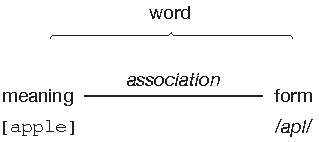
\includegraphics[width=0.35\textwidth]{figures/saussurean-sign}}}
  \caption{A diagram that illustrates our notion of the term ``word''
    as referring to the whole association of a meaning to a form.}
  \label{f:saussurean-sign}
\end{figure}

We have introduced the social context in which our communicative
interactions are going to take place. Next, we're going to define what
it means for our agents to ``know a language''. Since the focus of our
thesis is on lexicon formation (which leaves out many crucial aspects
of natural language such as grammar and morphology), our agents'
linguistic inventories are single \emph{lexicons}, consisting solely
of \emph{words}. Words are couplings between a \emph{meaning} and a
\emph{form} (see Figure \ref{f:saussurean-sign}) and we will
consistently use the term \emph{word} to refer to the whole of this
association (and not to the form). What meanings are and where they
come from will be the topic of the next Section \ref{s:meanings}. For
now we will treat them as sets of unstructured symbols (or
\emph{categories}, \emph{attributes}, \emph{features},
\emph{conceptual entities}, whatever you want to call them) such as
{\tt object-34}, {\tt category-17}, {\tt red-2} and so on. Forms are
random character strings that are created by speakers whenever they
invent a new word. Throughout our thesis, these forms will be built
from three random consonant/ vowel pairs such as for example in
``nuzega'' or ``firopa''.


\subsection{Saussurean signs}
\label{s:saussurean-signs}

For the coupling between meaning and form we rely on the concept of
the the \emph{Saussurean Sign} \citep{saussure67cours}. It is a
bi-directional relation between a concept (in the sense of some entity
of thought, \emph{signified}) and a form (a sound, a gesture, etc.,
\emph{signifier}). Bi-directional means that the same representation
is used to parse and produce utterances (which is not self-evident --
it is easy to imagine non-reciprocal communication systems in which
agents use different representations for parsing and producing or in
which agents lack the capability to either parse or produce). The
connection between the signified and the signifier is arbitrary, i.e.
there is nothing in the concept of a donkey that determines the sound
``donkey'' (in fact, different cultures arbitrarily connect very
different forms to similar concepts of donkeyness, e.g. ``Esel'' in
German). It's important to note that Saussurean Signs don't link
actual sounds waves to physical objects existing in the world but both
the signifier and the signified are mental patterns of reoccurring
sensory experiences of sounds and objects. Furthermore, and this will
be more clear later on, it is not the signs directly that determine
what we speak or how we interpret utterances -- it is the differences
in meaning and form between within a whole system of signs that govern
the speech of individuals (\emph{parole} in Saussure's terms). That
is, speakers don't follow explicit rules (in a classical artificial
intelligence rule system sense) such as {\tt \ "if donkey visible
  $\rightarrow$ produce sound `donkey'"} -- instead, they consider
their whole system of signs and their differences in meaning to
eventually use the sign that \emph{distinguishes} the donkey from
the other objects in the scene.

We'll assume Saussurean signs to be an appropriate construct for the
representation of form-meaning couplings in our work (especially the
notion of bi-directionality, arbitrariness and the importance of
relative differences to other signs), and we think that this is not a
controversial choice. But there is still the question of where this
particular nature of words comes from. To investigate this,
\cite{hurford89biological} compared different strategies for lexicon
formation in computer simulations. Learners either separately imitated
the production and speaking behavior of others or used observed
speaking behavior both in production and interpretation. The latter
strategy clearly had advantages because it makes it easier for the
agents to learn. Additionally, \cite{oliphant96dilemma} carried out
similar simulation studies which demonstrated that Saussurean
communication is favourable in populations of repeatedly interacting
agents (e.g. as in our language games), especially when the
populations are spatially organized. These experiments clearly show
that the Saussurean nature of words has advantages over other
communication systems. But the authors discuss these results under the
assumption that Saussurean communication evolved by means of natural
selection, a view that is challenged nowadays (see
\citealp[pp. 74--78]{bloom00how-children} for a discussion). As an
alternative, the bi-directional use of signs can be seen as a
consequence of our theory of mind: ``Children's ability to reproduce
intentional communicative actions via some form of cultural or
imitative learning involves a role reversal -- the child has
intentions towards the other person's intentional states -- which
leads to the creation of linguistic conventions''
\citep[p. 153]{tomasello01perceiving}. So we don't directly imitate
the linguistic behavior of others, that is, we don't imitate the
production of the sound ``donkey'' in the presence of a donkey but we
imitate the action of saying ``donkey'' as a method for directing
attention to donkeys. ``Once a child believes that the adult's use of
the word \emph{dog} was used with the intent to refer to a dog, then
she could use the same means (saying `dog') to satisfy this goal''
\citep[p. 76]{bloom00how-children}.

Finally, how are we going to implement our agents' systems of
Saussurean signs in terms of data structures? We'll choose the most
simple representation possible: a lexicon is represented as a list of
words, each having a meaning, a form and a score reflecting how
successful that word was used in past interactions. As we will see
later, the lexicon is usually part of a larger \emph{semiotic
  network}, a complex network \citep{strogatz01exploring} that
connects an agent's sensory experiences to forms and back and whose
overall behavior is the result of a coupling of different processes
that each have their own dynamics. There are many representations
thinkable that are more cognitively plausible than lists of words. For
example \cite{kosko88bidirectional} implemented a two-layer neural
network that can store paired data associations and
\cite*{billard99drama} developed DRAMA (dynamical recurrent
associative memory architecture) specifically for representing words
in robots. We prefer our representation over more integrated solutions
because it gives us full control over processes of language use and
learning. We assume that these structures could be easily transferred
into more natural representations (e.g. neural networks).


\subsection{Increasing complexity in the coupling between form and
  meaning}
\label{s:nature-of-form-meaning-couplings}


Words are couplings between meaning and form. We'll treat forms as
simple random strings and what meanings are will be explained in the
next section. We will turn now to the nature of this coupling, i.e.
how a form is coupled to meaning and how words in a lexicon relate to
each other. This structure is part of an agents cognitive
infrastructure, especially his mechanisms for production/
interpretation, learning and alignment. And it has direct consequences
on the dynamics of the language game experiments, i.e. how quick the
agents reach communicative success and coherence. Depending on the
``degrees of freedom'' in what the agents can associate to a form, in
how words with equivalent meanings/forms relate to each other, and in
how agents combine different words into utterances, various kinds (and
degrees) of \emph{ambiguities} arise in an agent's lexicon. For
example in all of these models it happens that different forms for the
same meaning spread in the population (because agents independently
invent them), causing \emph{synonyms} (the same meaning is associated
to multiple forms) to occur in the agent's lexicon. Similarly,
different contexts and other reasons might cause an agent to adopt
multiple meanings to the same form (\emph{homonymy}).

What does it mean for an agent to have for example a synonym in his
lexicon? Technically, an agent that learnt two different forms $f_1$
and $f_2$ for the meaning $m_1$ will not store them in the same word
with connections to both forms, but he maintains two separate
representations $w_1: m_1 \Leftrightarrow f_1$ and $w_2: m_1
\Leftrightarrow f_2$. Part of the self-organization process in the
series of language games is that the whole population eventually
agrees on one single form for a particular meaning (and vice
versa). In order to reach this goal, each agent individually tries to
optimize his own lexicon by preferring the most conventionalized
associations and eliminating \emph{competing} synonymous and
homonymous words. We will introduce various algorithms that achieve
this -- all of them rely on scoring each word depending on how
successful it is used in communication. When enough agents in the
population start preferring a particular form-meaning association, it
will prevail over the others, causing each individual agent to remove
competing synonyms and homonyms.

\begin{figure}[t]
\centerline{
\begin{tabular}{lp{0.7cm}l}
 A & & B \\
 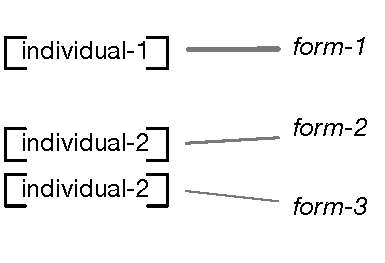
\includegraphics[width=0.31\columnwidth]{figures/models-of-form-meaning-couplings-1} & &
 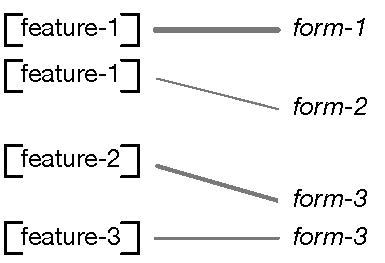
\includegraphics[width=0.31\columnwidth]{figures/models-of-form-meaning-couplings-2} \\
 & & \\
 C & & D \\
 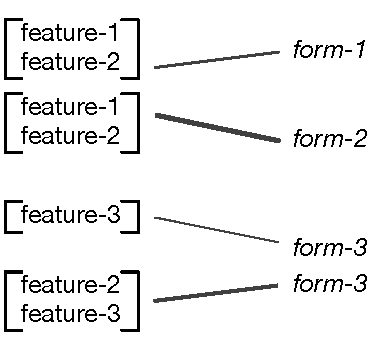
\includegraphics[width=0.31\columnwidth]{figures/models-of-form-meaning-couplings-3} & &
 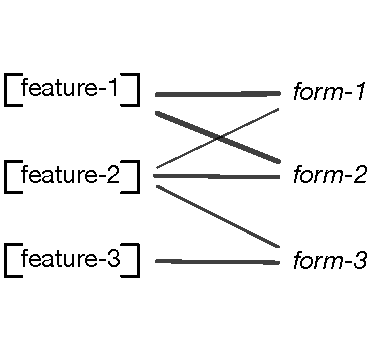
\includegraphics[width=0.31\columnwidth]{figures/models-of-form-meaning-couplings-4} 
\end{tabular}}
\caption{Increasing complexity in the nature of the coupling between
  form and meaning.  Hypothetical example lexicons of one agent are
  shown for four different models of lexicon formation.  Line widths
  denote different connection weights (scores).  A: One-to-one
  mappings between names and individuals in the Naming Game. There can
  be competing mappings involving the same individual (synonyms). B:
  One-to-one mappings between words and single categories in Guessing
  Games. Additionally to synonymy, there can be competing mappings
  involving the same words (homonymy). c: Many-to-one mappings between
  sets of categories and words. In addition to synonymy and homonymy,
  words can be mapped to different competing sets of categories that
  partially overlap each other. D: Flexible word meaning
  representations. Competition is not explicitly represented but words
  have flexible associations to different categories that are shaped
  through language use.
}
\label{f:models-of-form-meaning-couplings}
\end{figure}

Furthermore, other ambiguities arise from the use of \emph{multi-word}
utterances (it can become unclear which word covers which meaning),
from \emph{specificity} relations (whether a new word refers to the
whole object, to it's kind or a general property of it), and others.
The degrees of freedom in what to associate to a new form can be
interpreted as the \emph{complexity} of a lexicon formation model and
we will classify a variety of models according this degree of
freedom. For now, Figure \ref{f:models-of-form-meaning-couplings}
illustrates the nature of the coupling between meaning and form for
four of them.

The simplest of these four models, the \emph{Naming Game}
(\citealp{steels95selforganizing,steels99spatially}; Figure
\ref{f:models-of-form-meaning-couplings}A), is historically also the
oldest. The task in this game is to agree on a set of names for
established individuals (for example proper names such as ``John'' and
``Mary'' for individual persons).  Agents jointly perceive sets of
uniquely identifiable objects such as for example {\tt object-3}, {\tt
  object-8}, {\tt object-4}; or (as in
\citealp{steels95selforganizing}) unambiguously interpretable
positions on a spatial grid relative to the speaker (e.g. {\tt front},
{\tt side}, {\tt behind}, {\tt left}, etc). Words are thus one-to-one
associations between a representation for an individual and a name.
Since both speaker and hearer have the same representations of
individuals (the world they perceive consists already of
pre-conceptualized symbolic representations for unique objects or
locations), the hearer immediately knows which concept to associate to
a novel word after the speaker pointed to it. But synonymy can occur
because different speakers might invent different names for the same
object (for example in Figure
\ref{f:models-of-form-meaning-couplings}A the words {\tt
  individual-2}$\Leftrightarrow$\emph{form-2} and {\tt
  individual-2}$\Leftrightarrow$\emph{form-3} are synonymous).


Figure \ref{f:models-of-form-meaning-couplings}B illustrates a next
class of models. It is commonly referred to as a \emph{Guessing Game}
and was first introduced by \cite{steels96emergent}. It takes away the
scaffold that objects are represented as unique concepts by letting
the agents perceive scenes in which objects are sets of
pre-conceptualized discrete categories as for example in:
\begin{verbatim}
object-1: [weight heavy] [size medium] [shape square]
object-2: [weight light] [size small] [shape round]
object-3: [weight heavy] [size tall] [shape square]
\end{verbatim}
\noindent The speaker then searches for a category that
\emph{discriminates} the chosen topic from the other objects in the
context (for example {\tt [size medium]} discriminates {\tt object-1}
from the rest, {\tt [weight light]} or {\tt [shape round]}
discriminate {\tt object-2}, etc.) and then uses a single word to
express that meaning (the game stops when no discriminative category
can be found). So the words acquired by the agents are comparable to
adjectives for basic categories such as ``red'', ``small'' or
``round''. The representation of words is identical to those of Naming
Games (a one-to-one mapping between an atomic category and a form), but
further difficulties arise because the hearer does not know which
sensory quality (or channel) a novel word refers to. Consequently,
homonyms may appear in addition to synonyms because a hearer might
adopt different interpretations of the same word (for example in the
agent in Figure \ref{f:models-of-form-meaning-couplings}B interprets
the form \emph{form-3} both as {\tt feature-2} and as {\tt
  feature-3}). Because the words in this game still ``name'' single
categories, such experiments are sometimes called Naming Games as
well, reserving the term Guessing Game for the language game script.

\cite{looveren99multiple,looveren00analysis} presented two further
innovations: first, \emph{multi-word} utterances were introduced:
objects don't need to be discriminated anymore by a single category
but combinations of categories can be expressed by different words
(e.g. ``red'' and ``small'' when some other objects in the context are
also red and some others also small, but none of them red and small at
the same time). This leads to the additional difficulty that when a
hearer is confronted with two novel words at the same time then he
does not know which word covers which part of the inferred meaning
(such a situation is usually seen as too difficult: hearers only learn
when there is only one unknown word so that they can infer its meaning
using the know words and the context). Second, meanings of words can
be \emph{structured}: instead of expressing a single individual or
category, words are many-to-one mappings between forms and sets of
discrete categories (see Figure
\ref{f:models-of-form-meaning-couplings}C). Due to this, another
challenge arises for the hearer: he does not know to which subset of
the topic's feature he has to associate a new word. As a result, the
agents' lexicons do not only contain homonyms but also competing words
where the meaning of one is the subset of another (e.g. in Figure
\ref{f:models-of-form-meaning-couplings}C there are two words with the
form \emph{form-3}: one that expresses only {\tt feature-3} and one
that covers both {\tt feature-2} and {\tt feature-3}).


In order to scale up the above three lexicon formation models towards
more complex meaning spaces and in order to allow for the emergence of
more natural communication systems,
\cite*{wellens08flexible,wellens12multi-dimensional} proposed another
lexicon representation as shown in Figure
\ref{f:models-of-form-meaning-couplings}D. The main innovation is to
tackle ambiguities in what words mean with a \emph{flexible} coupling
between meaning and form: whereas agents in the previous models try to
figure out the meaning of a word by adopting multiple associations
between a form and its alternative meanings (and then use word scoring
techniques to rule out all of them except one), here the uncertainty
is put in the word representation itself. Instead of having a single
score for the whole coupling between a form and a set of categories,
each connection to a category is scored separately, which allows the
meaning of a word to gradually change towards its conventional use in
the population. Figure \ref{f:models-of-form-meaning-couplings}D tries
to illustrate this: an agent's lexicon is represented as a
many-to-many association between categories and forms, with each
connection scored separately.




\section{Meanings: grounded word semantics}
\label{s:meanings}

In addition to the social context of the communicative interactions
and the nature of word representations, the notion of ``meaning'' is
central to the understanding of communication in general and models
lexicon formation in particular. In our simulated language game
experiments, as discussed before, the world of the agents already
provides shared pre-conceptualized meanings consisting of (sets of)
symbols such as {\tt object-34}, {\tt category-17} or {\tt
  red-2}. With the meanings already being ``in the world'', they are
also immediately shared by all agents in the population and the
question what meanings are and where they come from is not posed --
the focus is rather on reaching consensus on which meanings to connect
to which forms. However, objects in the real world -- which is also
the world of our robots -- do not come with universally shared
properties directly accessible to observers. Instead, each agent has
to construct ``meanings'' as his own interpretation of a scene from
its sensori-motor interaction with the environment.



\subsection{From Saussure to Peirce}
\label{s:saussure-to-peirce}


A widely accepted notion of meaning is that they are not something to
be found in the world, but that they are used to \emph{refer} to
things in the world: ``The traditional view, emerging first in
Aristotle, is that the meaning of a word is what determines its
reference. ... Hence the meaning of \emph{dog} determines which things
are and are not dogs, and knowing the meaning of dog entails knowing
what things are dogs and are not dogs''
\citep[p. 18]{bloom00how-children}.

\begin{figure}
  \parbox{0.6\textwidth}{\centerline{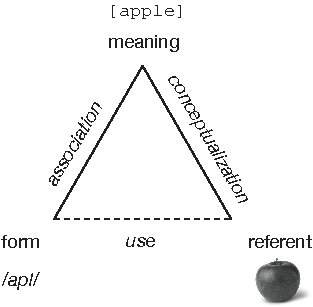
\includegraphics[width=0.4\textwidth]{figures/semiotic-triangle}}}
  \caption{Diagram of a semiotic triangle. The relation between a
    meaning, a form and a referent loosely resemble the definition of
    a sign by \cite{peirce31collected}. }
\label{f:semiotic-triangle}
\end{figure}


Adding referents to De Saussure's (\citeyear{saussure67cours}, see
also Section \ref{s:saussurean-signs} above) definition of a sign as a
relation between a meaning and a form, \cite{peirce31collected}
introduced the concept of a sign as a triadic relationship between a
form, a meaning and a referent (see Figure
\ref{f:semiotic-triangle}). Peirce originally used the term
\emph{representamen} for the \emph{shape} (form) of the sign and
\emph{interpretant} for its \emph{sense} or \emph{concept} (meaning).
For the referent, which is a physical object in the world but which
also can be abstract, Peirce used the term \emph{object}. 


The relation between form an meaning is, analogous to the Saussurean
sign, an arbitrary conventionalized bi-directional association between
a meaning and a form. And although finding the appropriate meaning
underlying a form or finding the form that expresses a meaning of
course requires some look-up process, these associations can be
considered to be ``stored'' in the lexicon of an agent. In contrast,
the relation between meanings and referents is of a different
nature. Word meanings are representations that allow to determine to
which referents a word applies and to which not. Therefore, finding
out whether a specific meaning is applicable to a specific referent in
the context is an active process that in each interaction again
establishes the relation between a meaning and a referent. We call the
process of determining the meanings that are applicable to a referent
\emph{conceptualization} and the reverse process of applying the
meanings underlying an utterance to a situation in order to determine
a referent \emph{interpretation}.


The third relation in Figure \ref{f:semiotic-triangle} between forms
and referents is even less direct. The meaning representations
maintained by each agent are not accessible by other agents -- they
can only observe forms and referents. Meanings thus constitute an
intermediate layer that allows agents to relate the same words to
similar referents in the world, i.e. \emph{use} a word in the same
way: ``For a large class of cases -- though not for all -- in which we
employ the word `meaning' it can be defined thus: the meaning of a
word is its use in the language'' \citep[Part I, Section
43]{wittgenstein67philosophische}. For example, the meaning of ``red''
is a shared convention how to classify the world into things that are
red and things that are not. Moreover, meaning representations are
constructed individually by each agent from sensory experiences of
specific referents. And because every agent has a different history of
interactions with the world and other agents, two agents will never
connect exactly the same meaning representation to the same
form. Intuitively, every two humans will also have slightly different
opinions about which border cases of red objects should be considered
red, but they will still use ``red'' successfully in most of the cases
to refer to red object. As we will see later, conceptual coherence,
i.e. the similarity between meanings acquired by different agents, is
not necessarily a prerequisite for successful communication. It is
enough that we all use a word to refer to the same things -- further
cognitive overlap is not necessary.


Furthermore, conceptualizing a referent or interpreting a meaning
never happens in a vacuum. Words can be used differently in different
contexts (for example ``the red block'' can be used to refer to an
orange block when all other objects are blue, but not when there is
another red block). And more importantly, the interpretation of words
depends also on the social context, i.e. the previous discourse and
the kind of communicative interaction. As discussed above in Section
\ref{s:language-game}, the language game played determines how words
have to be interpreted to yield a referent. ``We must therefore
explicitly acknowledge the theoretical point that linguistic reference
is a \emph{social} act in which one person attempts to get another
person to focus her attention on something in the world''
\citep[p. 97]{tomasello99cultural}. In our experiments, the type of
communicative interaction is fixed (see Figure
\ref{f:guessing-game-flow}, page \pageref{f:guessing-game-flow}) and
the implicit communicative goal underlying each utterance is to draw
attention to a single object in the environment of the
robots. Consequently, when an agent says for example ``red small'',
then the built-in convention is to interpret these words as ``please
point to the object that is small and red''.


The question of how to represent and process word meanings is very
closely related to the \emph{symbol grounding problem}
\citep{harnad90symbolgrounding}, which his ``... , generally speaking,
the problem of how to causally connect an artificial agent with its
environment such that the agent's behavior, as well as the mechanisms,
representations, etc. underlying it, can be intrinsic and meaningful
to itself, rather than dependent on an external designer or observer''
\citep[p.~177]{ziemke99rethinking}. The debate around this problem was
started by \cite{searle80minds} with the Chinese room argument as a
critique to early paradigms in artificial intelligence that envisioned
the possibility of intelligence based solely on the manipulation of
idealized \emph{physical symbol systems}
\citep{newell76computer,newell80physical} and since that has occupied
many philosophers and cognitive scientists. However, when adopting the
notion of meaning discussed above as a functional relation between
forms, internal representations and referents, then ``... one may
argue that argue that the semiotic symbol is \emph{per definition}
grounded, becasue the triadic relation (i.e. the semiotic symbol)
already bears symbols meaning with respect to reality''
\citep[p.~434]{vogt02physical}. We will thus not take part in this
debate and rather focus on the technical challenge of the acquisition
of meanings through the interaction of a physical body with the
environment and on processes for conceptualization and semantic
interpretation, which together ``solve the symbol grounding problem''
\citealp*{steels08symbol-grounding,steels07semiotic}.



\subsection{Mental representations for categorization}
\label{s:mental-representations-for-categorizations}

Peirce's definition of a sign can be discussed without subscribing to
any theory of what word meanings are and how they are represented in
an agent, a question which has occupied philosophers, logicians,
linguists and psychologists for a very long time. We will not delve
into the history of this debate but rather stick with contemporary
notions of meaning in the cognitive sciences that are based on the
concept of \emph{categories}, as advanced by scholars such as
\cite{lakoff87woman}, \cite{harnad87categorial} or
\cite{barsalou99perceptual}. A category is a representation that
allows to classify objects according to some criterion or ``a category
exists whenever two or more distinguishable objects or events are
treated equivalently'' \citep[p. 89]{mervis81categorization}. We call
the long-term memory of categories that are acquired by an agent an
\emph{ontology}.


Categories are abstractions from the continuous sensori-motor
interaction with the environment that have proved to be useful for an
agent, for example in communication: ``one purpose of categorization
is to reduce the infinite differences among stimuli to behaviorally
and cognitively usable proportions. It is to the organism's advantage
not to differentiate one stimulus from others when that
differentiation is irrelevant for the purposes at hand'' \citep[page
384]{rosch76basic}. Consequently, well-tuned category systems
contribute to the cognitive economy of an agent because they limit the
number of sensori-motor patterns that have to memorized and they can
be processed independently of the context in which they were created
and the objects and the events that they stand for, a phenomenon which
\cite{gardenfors05detachment} calls the ``detachment of
thought''. Finally, categories are not only used for language, but
also for a big variety of other cognitive activities such as for
example planning. Some scholars such as
Peirce~(\citeyear[p.~2.302]{peirce31collected}) even claim that ``we
think only in signs''.


Early psychological studies by \cite{rosch73natural} have shown that
many categories do not have strict borders but that membership to a
category is continuous. For example, the category \texttt{red} does
not unambiguously divide all things in the world into a set of objects
that are red and into another set of objects that are not red, but
instead provides a graded judgement of \emph{how} red an object
is. And at least for `basic level' categories, \cite{rosch73natural}
demonstrated that the gradedness of this classification is a function
of the similarity to a \emph{prototype}, which can be understood as a
point in a sensori-motor space that defines the center of the
category. Such a space is defined by multiple dimensions representing
continuous sensory or other qualities and multiple categories defined
by points in that space. For example color categories can be
represented as points in a two- or threedimensional color space and
color categorization of an object then means to find the category that
has the closest geometric distance to a stimulus. Along that line,
\cite{gardenfors00conceptual-spaces} introduced the theoretic
framework of `conceptual spaces' for an operationalized geometric
account of categorization and provided examples for many domains, such
as for example in \citep{gardenfors01reasoning}.\\


\noindent As mentioned before, we will not to equip our agents with pre-existing
engineered sets of categories but endow them with mechanisms for the
autonomous creation of truly grounded ontologies. For that, most work
on category formation in the field of artificial intelligence has been
done (very successfully) using techniques of machine learning
\citep{mitchell97machine}. Such learning methods always require data
sets of example stimuli together with their correct classification
(usually labelled manually by a human) and then a classifier (for
example based on a neural network or a K-nearest neighbor algorithm)
is trained so that it eventually can reproduce the classificaton that
is implicit in the example set. However, there are three problems with
such approaches: First, in open-ended interaction and learning
scenarios where the things to expect in the environment are not known
in advance, proper training sets may not be easily available at all.
Second, once classifiers are trained, they don't adapt and thus the
learnt classification may become inappropriate when new types of
objects occur in the environment (which is the case for humans and for
our robots). And third, the categories learnt with machine learning
techniques are still induced by a designer because he used his own
(human) category system to create the labelled data sets. For a
further discussion of the problems involved in applying machine
learning techniques to autonomous category formation, refer to
\citep{steels97constructing}.


We will thus need mechanism that allow our agents to gradually
construct and shape their ontologies from the continuous interaction
with the environment and other agents, in a similar way to the
self-organization of lexicons discussed above. One method for this
introduced by \cite{steels96perceptually} are \emph{discrimination
  trees} (we will disscuss them in Chapter
\ref{c:grounded-categories}). He presented simulated agents with
generated contexts consisting of objects characterized by real-valued
features and in order to be successful in discriminating one object
from the other objects in such a generated context, they created
categories by further and further sub-dividing the range of feature
values into smaller and smaller regions (hence the term discrimination
tree).  Discrimination trees were then implemented by
\cite{steels97constructing,steels97grounding} on wheeled LEGO robots
to create categories for distances measured with infrared sensors and
later by
\citep{steels99situated,steels99collective,steels02bootstrapping} in
the Talking Heads experiment (discussed further below) for visual
features such as color, size and position obtained by pan-tilt cameras
directed at a whiteboard with objects. Also with LEGO robots,
\cite{vogt01bootstrapping,vogt03anchoring} conducted similar
experiments, but instead of discrimination trees, categories were
created as prototypes in the sensory space of a bigger range of
distance sensors. Finally, the formation of color categories using
various prototype-based approaches was studied extensively by
\cite{steels05coordinating} who presented agents with perceptions of
sets of color chips and by \cite*{bleys09grounded} who used the same
robotic setup with humanoid robots as in this thesis.




\subsection{Categories and language}

Because the agents in our experiments will construct and shape their
ontologies exclusively for the purpose of being successful in the
given task of communicating about objects in their environment, both
the adequateness of each agent's individual category system as well as
the coherence between different agents' ontologies directly have an
impact on the overall communicative success of the population, which
in return means that success in communication is a also a good measure
for driving the self-organization of the category
systems. Consequently, effective mechanisms for orchestrating the
co-evolution of conceptual and linguistic inventories through a tight
coupling are crucial for successful communication (see
\citealp{steels98origins-ontologies} for a discussion and review of
early experiments).

\begin{figure}[t]
  \centerline{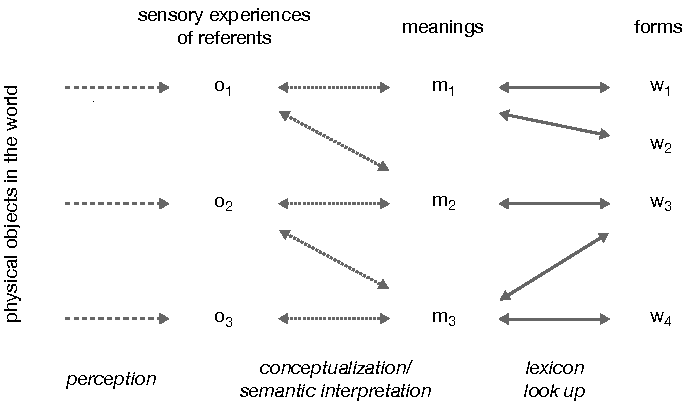
\includegraphics[width=0.75\textwidth]{figures/semiotic-network-example}}
  \caption{A schematic model of an agent's semiotic
    network. Perceptual processes yield representations of sensory
    experiences that then become connected to meaning representations
    through processes of conceptualization and semantic
    interpretation. Forms are connected to meanings through a lexicon
    look up process.}
  \label{f:semiotic-network-example}
\end{figure}


The perceptual, conceptual and linguistic representations that are
maintained by each agent for producing and parsing utterances can be
viewed as a \emph{semiotic network} as shown in Figure
\ref{f:semiotic-network-example}. Long-term memories of meanings are
connected to forms through persistent associations that are stored in
the agent's lexicon. For production and parsing, a look up process
retrieves the best form connected a meaning and vice versa. In
contrast, representations of sensory experiences that are created by
perceptual processes for referents are only memorized over the course
of a single interaction. They become dynamically connected to meanings
through processes of conceptualization and semantic
interpretation. Each of the connections between representations in a
semiotic network is weighted. Scores of form meaning associations
reflect how well a word was used in the past and conceptualizations
are scored based both on how well a category discriminates a referent
from the context and on success in previous interactions. Producing or
parsing an utterance then amounts to finding an optimal path through
the network, either by always following connection with highest weight
or by searching for the highest cumulative score.


The biggest challenge in maintaining semiotic networks lies the
coupling between the alignment dynamics of meanings and of words. The
communicative success perceived by an agent only provides an overall
measure for the appropriateness and degree of conventionalization of
all the representations along a particular path through the semiotic
network. For example when an interaction fails, an agent has no
guaranteed way of attributing the failure in order to repair its
network -- it could be both due to an inappropriate category, due to a
wrong word, or due to a disadvantageous connection weigth that
prevented the agent from using the `right' path through the network.
Similarly, also positive communicative feedback only acts on both the
involved categories and words and as we will see later on, it needs
many interactions to disentangle the fortune of particular categories
from those of the words connected to them.\\


\noindent By letting agents create and align meanings in a way so that
they fit well with the linguistic conventions in a population, we give
language a very prominent role in the formation of categories, which
is not an uncontroversial choice. Next to language that imposes and
structures concepts, there are at least two other important factors:
First, while it is very unlikely for most of the categories to be
innate, the genetic endowment of agents certainly constrains the
morphology of the body and its perceptual apparatus. And similar
sensori-motor interactions with the environment lead to a similar
structuring of reality. Second, the structure of the world itself also
constrains concept formation. Some patterns in the world occur more
often than others and some distinctions are more salient than others,
and for efficient communication it makes sense to reflect these
patterns in the language. How these three factors are weighted is an
ongoing debate in the cognitive sciences and we will not take a stance
in this discussion. In our experiments, language, the body and the
world play an equally important role.

Nevertheless, the previously unpopular theory of \emph{linguistic
  relativity} which proposes a strong influence of language on the
nature of categories (or Sapir-Whorf hypothesis,
\citealp{whorf56language}) started to receive more an more support
recently (see for example \citealp{levinson01language} for a review of
empirical evidence and arguments). And there is quite of number of
computational studies demonstrating that the shaping of categories
through language is beneficial for the self-organization of
communication systems. For example \citep{cangelosi02adaptive} showed
in an experiment where simulated agents were interacting in a
toy-world consisting of mushrooms (with some of them being poisonous)
that agents that have to construct their sensori-motor categories
solely by trial-and error interactions with the environment have an
evolutionary disadvantage compared to those whose categories are
shaped through language.


A related question is whether the learning of word meanings requires
the pre-existence of categories (learnt or innate) or whether, in the
other extreme, the mental world is exclusively structured through
language. In humans, linguistic development is preceded by a phase in
which mental representations are constructed solely from the
non-linguistic interaction with the world. However, concepts such as
number systems or as simple as color categories are clearly culturally
transmitted and thus even if language initially relies on pre-existing
representations, in later stages there is a co-evolution of categories
and words and we will also pursue that strategy in our experiments.
In support, \cite{clark04how} reviewed empirical evidence (for the
domain of space) on how children first build on conceptual
representations acquired in pre-linguistic stages and how these
representations are refined or build upon later when learning the
underlying representational structure of the parent's language.


Finally, the issue of planning and interpretating multi-word
utterances is also linked to the interplay between categories and
language. First of all, we need to define what the meaning of an
utterance is: in interpretation, it is the combined meanings of all
the words involved in parsing. Consequently, when an agent connects
many different meanigns to the same word forms, then many different
sets of categories can result from applying a lexicon. Semantic
interpretation of such a list of categories will then look for the
object that fits all categories best. In production, conceptualization
processes try to find a set of categories that disriminate the chosen
topic from the other objects in the context. Lexicon application then
needs to find a combination of words that \emph{cover} each of the
categories in the meaning, a process which again can yield multiple
combinations of words.

In general, agents trace their semiotic networks in parallel for the
involved representations and additional conceptualization and lexicon
processes need to check whether combined sets of categories and words
are applicable to a context, meaning or utterance. How exactly
linguistic and semantic representations are to be processed is
implicitely hidden in the language game and shared by all agents. For
advancing this work towards grammatical language, more explicit means
of representing how to apply categories are certainly needed and a
good candidate for this is the \emph{IRL} framework
\cite*{steels05planning,vandenbroeck08constraint-based,spranger10open-ended-semantics,spranger10open-ended,spranger12openended}
which enables agents to autonomously construct compositional semantic
structures that configure the interplay of cognitive categorization
operations and categories.






%%% Local Variables: 
%%% mode: latex
%%% TeX-master: "phdbook"
%%% End: 
